%%%%%%%%%%%%%%%%%%%%%%%%%%%%%%%%%%%%%%%%%
% Beamer Presentation
% LaTeX Template
% Version 1.0 (10/11/12)
%
% This template has been downloaded from:
% http://www.LaTeXTemplates.com
%
% License:
% CC BY-NC-SA 3.0 (http://creativecommons.org/licenses/by-nc-sa/3.0/)
%
%%%%%%%%%%%%%%%%%%%%%%%%%%%%%%%%%%%%%%%%%

%----------------------------------------------------------------------------------------
%	PACKAGES AND THEMES
%----------------------------------------------------------------------------------------

\documentclass{beamer}

\mode<presentation> {

% The Beamer class comes with a number of default slide themes
% which change the colors and layouts of slides. Below this is a list
% of all the themes, uncomment each in turn to see what they look like.

\usetheme{default}
%\usetheme{AnnArbor}
%\usetheme{Antibes}
%\usetheme{Bergen}
%\usetheme{Berkeley}
%\usetheme{Berlin}
%\usetheme{Boadilla}
%\usetheme{CambridgeUS}
%\usetheme{Copenhagen}
%\usetheme{Darmstadt}
%\usetheme{Dresden}
%\usetheme{Frankfurt}
%\usetheme{Goettingen}
%\usetheme{Hannover}
%\usetheme{Ilmenau}
%\usetheme{JuanLesPins}
%\usetheme{Luebeck}
%\usetheme{Madrid}
%\usetheme{Malmoe}
%\usetheme{Marburg}
%\usetheme{Montpellier}
%\usetheme{PaloAlto}
%\usetheme{Pittsburgh}
%\usetheme{Rochester}
%\usetheme{Singapore}
%\usetheme{Szeged}
%\usetheme{Warsaw}

% As well as themes, the Beamer class has a number of color themes
% for any slide theme. Uncomment each of these in turn to see how it
% changes the colors of your current slide theme.

%\usecolortheme{albatross}
%\usecolortheme{beaver}
%\usecolortheme{beetle}
%\usecolortheme{crane}
%\usecolortheme{dolphin}
%\usecolortheme{dove}
%\usecolortheme{fly}
%\usecolortheme{lily}
%\usecolortheme{orchid}
%\usecolortheme{rose}
%\usecolortheme{seagull}
%\usecolortheme{seahorse}
%\usecolortheme{whale}
%\usecolortheme{wolverine}

%\setbeamertemplate{footline} % To remove the footer line in all slides uncomment this line
%\setbeamertemplate{footline}[page number] % To replace the footer line in all slides with a simple slide count uncomment this line

%\setbeamertemplate{navigation symbols}{} % To remove the navigation symbols from the bottom of all slides uncomment this line
}

\usepackage{graphicx} % Allows including images
\usepackage{booktabs} % Allows the use of \toprule, \midrule and \bottomrule in tables

%----------------------------------------------------------------------------------------
%	TITLE PAGE
%----------------------------------------------------------------------------------------

\title[GAI based on ML]{General Game AI Based On Machine Learning} % The short title appears at the bottom of every slide, the full title is only on the title page

\author{maywzh} % Your name
\institute[JI] % Your institution as it will appear on the bottom of every slide, may be shorthand to save space
{
CCNU-UOW JI \\ % Your institution for the title page
\medskip
\textit{maywzh@gmail.com} % Your email address
}
\date{\today} % Date, can be changed to a custom date

\begin{document}

\begin{frame}
\titlepage % Print the title page as the first slide
\end{frame}

\begin{frame}
\frametitle{Overview} % Table of contents slide, comment this block out to remove it
\tableofcontents % Throughout your presentation, if you choose to use \section{} and \subsection{} commands, these will automatically be printed on this slide as an overview of your presentation
\end{frame}

%----------------------------------------------------------------------------------------
%	PRESENTATION SLIDES
%----------------------------------------------------------------------------------------

%------------------------------------------------
\section{Problem} % Sections can be created in order to organize your presentation into discrete blocks, all sections and subsections are automatically printed in the table of contents as an overview of the talk
%------------------------------------------------

\subsection{Introduction} % A subsection can be created just before a set of slides with a common theme to further break down your presentation into chunks

\begin{frame}
\frametitle{Introduction}
Tradationally, Game artificial intelligence (AI) refers to pre-defined automation programs generating adaptive or certain behaviors in fixed pattern for Non-player characters (NPCs) to simulate the reality in a real world.\cite{1}

Recently, the merge between academia and industry introduce machine learning algorithms and methods to video game AI development.\cite{2} This trend enhanced the AI capability to a large extent and can be positive for creating comparative adaptive and intelligent Game AI agents including NPC, intelligent machine players or even powerful General Video Game Playing AI (GVGAI), etc. 
\end{frame}

%------------------------------------------------
\subsection{Game AI Aims}
\begin{frame}
\frametitle{Game AI Aims}
\begin{itemize}
\item play certain or uncertain games as a player
\item without any human intervention
\item learn automatically to get better performance
\end{itemize}
\end{frame}

%------------------------------------------------
\subsection{Flagships}
\begin{frame}
\frametitle{Flagships\cite{2}}
\begin{block}{Player Experience Modeling\cite{3}}
  Player experience modeling (PEM) is the study and use of
  AI techniques for the construction of computational models
  of experience of players. 
\end{block}

\begin{block}{Procedural Content Generation\cite{4}}
  Generate playable, smooth, superior environment or game objects for game.
\end{block}


\begin{block}{Massive-Scale Game Data Mining\cite{5,6}}
  Data mining for player data to track these things:how. why , what do players play? To offer data analysis for game playing.
\end{block}

\begin{block}{NPC AI\cite{7,8,9}}
  Enhance the NPC capabilities and apply difficulty scaling techniques to this to improve the playing experience.

\end{block}
\end{frame}


%------------------------------------------------
\subsection{Game AI Learning problems}
\begin{frame}
\frametitle{Game AI Learning problems}
\begin{columns}[c] % The "c" option specifies centered vertical alignment while the "t" option is used for top vertical alignment

\column{.45\textwidth} % Left column and width
\textbf{Learning for Game AI\cite{10}}
\begin{enumerate}
\item Learning to play the game
\item Learning about players
\item Behavior capture of players
\item Model selection and stability
\item Optimizing for adaptivity
\item Model interpretation
\item Performance
\end{enumerate}

\column{.5\textwidth} % Right column and width
\begin{figure}
  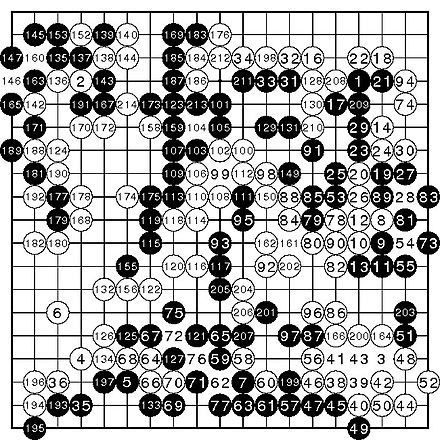
\includegraphics[width=0.8\linewidth]{figure/alphago}
  \caption{AlphaGo vs Fan Hui, Game 5}
\end{figure}
\end{columns}
\end{frame}

%------------------------------------------------
\section{Applications}
%------------------------------------------------
\subsection{AlphaGo}
\begin{frame}
  \frametitle{AlphaGo - Neural Network and Tree Search}
  Sliver et.al. \cite{11} introduce a new approach to computer Go that uses ‘value networks’ to evaluate board positions and ‘policy networks’ to select moves.
  \begin{figure}
    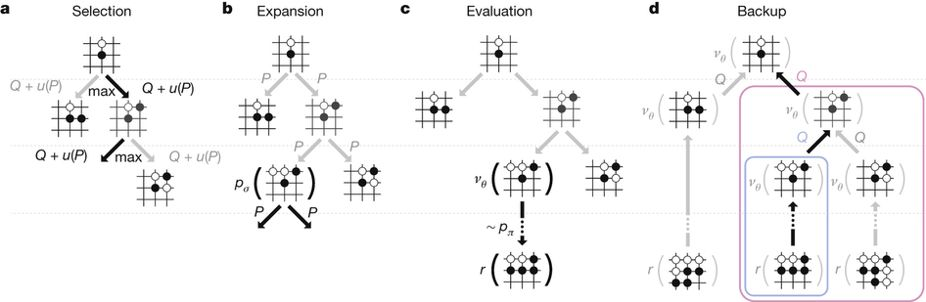
\includegraphics[width=1\linewidth]{figure/gosearch}
    \caption{ Monte Carlo tree search in AlphaGo}
  \end{figure}
\end{frame}

\subsection{StarCraft}
\begin{frame}
  \frametitle{Reinforcement Learning Applied to StarCraft}
  Wender and Watson did some research \cite{12} on applying reinforcement learning (RL) to tiny scale combat in StarCraft, aiming to design an agent performing unsupervised learning in complex environment. The result showed the viability of RL algorithms in SC.
  \begin{figure}
    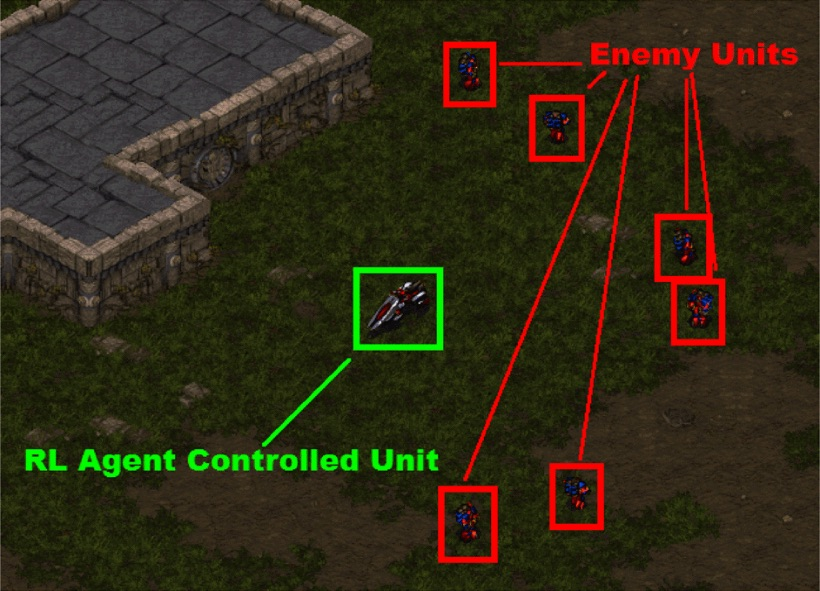
\includegraphics[width=0.6\linewidth]{figure/sc}
    \caption{ Initial unit positioning for the experimental evaluation}
  \end{figure}
\end{frame}

\subsection{Atari Games}
\begin{frame}
  \frametitle{Deep Reinforcement Learning Applied to Atari Games}
  Mnih et.al \cite{13} applied convolutional neural network trained with a variant of Q-learning to seven Atari 2600 games from the Arcade Learning Environment. The AI reached the expert level of human-like player.
  \begin{figure}
    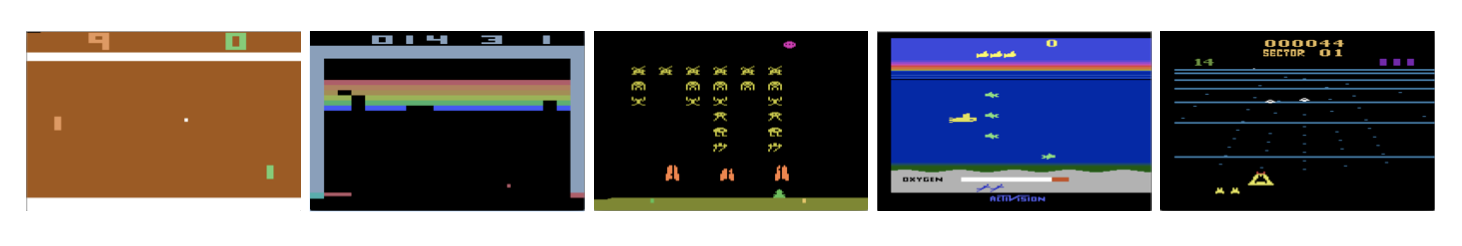
\includegraphics[width=1\linewidth]{figure/atari}
    \caption{  Screen shots from five Atari 2600 Games: (Left-to-right) Pong, Breakout, Space Invaders, Seaquest, Beam Rider}
  \end{figure}
\end{frame}
%------------------------------------------------



%------------------------------------------------

\begin{frame}[allowframebreaks]
\frametitle{References}
\footnotesize{
\begin{thebibliography}{0} % Beamer does not support BibTeX so references must be inserted manually as below

\bibitem{1}
Geogios~N Yannakakis.
\newblock Game ai revisited.
\newblock In {\em Proceedings of the 9th conference on Computing Frontiers},
  pages 285--292. ACM, 2012.
\bibitem{2}
Diego Perez-Liebana, Spyridon Samothrakis, Julian Togelius, Tom Schaul, and
  Simon~M Lucas.
\newblock General video game ai: Competition, challenges and opportunities.
\newblock In {\em Thirtieth AAAI Conference on Artificial Intelligence}, 2016.

\bibitem{3}
J. Juul.
\newblock A Casual Revolution: Reinventing Video Games and Their Players.
\newblock MIT Press, 2009.

\bibitem{4}
G. N. Yannakakis and J. Togelius.
\newblock Experience-Driven Procedural Content Generation.
\newblock In {\em IEEE Transactions on Affective Computing}, 2:147–161, 2011.

\bibitem{5}
  David Silver, Julian Schrittwieser, Karen Simonyan, Ioannis Antonoglou, Aja
    Huang, Arthur Guez, Thomas Hubert, Lucas Baker, Matthew Lai, Adrian Bolton,
    et~al.
  \newblock Mastering the game of go without human knowledge.
  \newblock {\em Nature}, 550(7676):354, 2017.
  
\bibitem{6}
Mark~Owen Riedl and Alexander Zook.
\newblock Ai for game production.
\newblock In {\em 2013 IEEE Conference on Computational Inteligence in Games
  (CIG)}, pages 1--8. IEEE, 2013.
  
\bibitem{7}
Alexander Nareyek.
\newblock Ai in computer games.
\newblock {\em Queue}, 1(10):58, 2004.
  
\bibitem{8}
Mark~Owen Riedl and Alexander Zook.
\newblock Ai for game production.
\newblock In {\em 2013 IEEE Conference on Computational Inteligence in Games
  (CIG)}, pages 1--8. IEEE, 2013

\bibitem{9}
David Conroy, Peta Wyeth, and Daniel Johnson.
\newblock Modeling player-like behavior for game ai design.
\newblock In {\em Proceedings of the 8th International Conference on Advances
  in Computer Entertainment Technology}, page~9. ACM, 2011.

\bibitem{10}
Michael Bowling, Johannes F{\"u}rnkranz, Thore Graepel, and Ron Musick.
\newblock Machine learning and games.
\newblock {\em Machine learning}, 63(3):211--215, 2006.


\bibitem{11}
David Silver, Aja Huang, Chris~J Maddison, Arthur Guez, Laurent Sifre, George
  Van Den~Driessche, Julian Schrittwieser, Ioannis Antonoglou, Veda
  Panneershelvam, Marc Lanctot, et~al.
\newblock Mastering the game of go with deep neural networks and tree search.
\newblock {\em nature}, 529(7587):484, 2016.

\bibitem{12}
S.~{Wender} and I.~{Watson}.
\newblock Applying reinforcement learning to small scale combat in the
  real-time strategy game starcraft:broodwar.
\newblock In {\em 2012 IEEE Conference on Computational Intelligence and Games (CIG)}, pages 402--408, Sep. 2012.

\bibitem{13}
Volodymyr Mnih, Koray Kavukcuoglu, David Silver, Alex Graves, Ioannis
  Antonoglou, Daan Wierstra, and Martin Riedmiller.
\newblock Playing atari with deep reinforcement learning, 2013.


\end{thebibliography}
}


\end{frame}


%------------------------------------------------

\begin{frame}
\Huge{\centerline{The End}}
\end{frame}

%----------------------------------------------------------------------------------------

\end{document} 